\documentclass[a4paper,twoside,onecolumn,openany,article,10pt]{memoir}
\usepackage{xeCJK}
\usepackage{url}
\usepackage{hyperref}
\usepackage{amsmath}
\usepackage{amssymb}
\usepackage{amsthm}
\usepackage{enumerate}
%\usepackage{algorithm}
%\usepackage{algorithmicx}
%\usepackage{algpseudocode}
\usepackage{ascmac}
\usepackage{tikz}
\usepackage{ulem}
%\usepackage{stix}
%\usepackage{bm}
\defaultfontfeatures{Ligatures=TeX}

\setCJKmainfont[BoldFont=Noto Sans CJK JP Bold]{Noto Serif CJK JP}
%\setCJKmainfont{Noto Serif CJK JP}
\setCJKsansfont{Noto Sans CJK JP}
\setCJKmonofont{Noto Sans Mono CJK JP}

\newtheorem{theorem}{定理}
\theoremstyle{remark}
\newtheorem{remark}{\textbf{余談}}


%\setmainfont{DejaVu Serif}
%\setsansfont{URW Gothic}
%\setmainfont{Noto Serif CJK JP}
\setmainfont[BoldFont=Noto Sans CJK JP Bold]{Noto Serif CJK JP}
\setsansfont{Noto Sans CJK JP}
\setmonofont{Inconsolata}

\usepackage{listings}

%\renewcommand{\algorithmcfname}{アルゴリズム}



\settrimmedsize{\stockheight}{\stockwidth}{*}

%\setlrmarginsandblock{1.5in}{1in}{*}
\setlrmarginsandblock{1.0in}{1.0in}{*}
\setulmarginsandblock{1.2in}{1.5in}{*}
\setheadfoot{20mm}{15mm}

%\newlength{\linespace}
%\setlength{\linespace}{\baselineskip}
%\setlength{\headheight}{\onelineskip}
%\setlength{\headsep}{\linespace}
%\addtolength{\headsep}{-\topskip}

%\setlength{\footskip}{\onelineskip}
%\setlength{\footnotesep}{\onelineskip}

\checkandfixthelayout

\counterwithout{section}{chapter}
\setsecnumdepth{subsubsection}


\title{アルゴリズムとデータ構造\\\vspace{.5em} \Large 二分探索}
%\date{2018年6月15日}
\date{}
\author{森~立平\\ \texttt{mori@c.titech.ac.jp}}

\begin{document}
\maketitle


\noindent
今日のメッセージ
\begin{itemize}
\item \textbf{ソートしてある配列から値を探すときは二分探索}
\item \textbf{二分探索の時間計算量は$O(\log n)$}
\item \textbf{単調な関数の逆関数を求める}ことに二分探索が使える
\end{itemize}

%\noindent
%今日の演習の目標
%\begin{itemize}
%\item 二分探索のプログラムを再帰、反復の両方で書けるようになる
%\end{itemize}
%
%\noindent
%今日の主な演習課題(提出締切は)
%\begin{enumerate}
%\item 二分探索のプログラムを書く
%\end{enumerate}
%
%\noindent
%今日の演習時間のワークフロー
%\begin{enumerate}
%\item GitHub のアカウントを取得し、Google Form で情報を送る(配布資料参照)
%\item \url{https://github.com/alg2018/} にアクセスし、\texttt{Algorithms--Datastructures}の「プログラミング演習のルール」を読む
%\item \url{https://github.com/alg2018/} にアクセスし、\texttt{GCD}にある課題に取り組む
%\item プログラムを紙に書いて教員かTAに提出
%\item \texttt{Algorithms--Datastructures/docs/git.pdf} を見て、\texttt{git}の使い方を覚える(来週以降に\texttt{git}を使用する)
%\end{enumerate}


\section{二分探索}
ソートしてある整数の列$A_0\le A_1\le A_2\le \dotsb\le A_{n-1}$の中から、$x$以上である最小のものを見つける問題を考えよう。
便宜上$A_n := +\infty$と定義し、
\begin{equation*}
\mathrm{bsearch}(\ell, r) := \min\bigl\{i\in\{\ell,\ell+1,\dotsc,r-1,r\}\mid A_i\ge x\bigr\}
\end{equation*}
と定義すると、解きたい問題は$\mathrm{bsearch}(0,n)$である(もしも$A_0$から$A_{n-1}$に$x$以上のものが無ければ$\mathrm{bsearch}(0,n)=n$となる)。
「アルゴリズム$\approx$漸化式」であるから、漸化式を立てることを考えよう。
\begin{equation*}
\mathrm{bsearch}(\ell, r) =
\begin{cases}
\ell,& \text{if } \ell = r\\
\mathrm{bsearch}(\lfloor \frac{\ell + r}2\rfloor+1, r),& \text{if } A_{\lfloor\frac{\ell + r}2\rfloor} < x\\
\mathrm{bsearch}(\ell, \lfloor \frac{\ell + r}2\rfloor),& \text{otherwise.}
\end{cases}
\end{equation*}
この漸化式に基づいてアルゴリズムを設計できる。

\begin{lstlisting}[basicstyle=\ttfamily\normalsize,showstringspaces=false,language=C,frame=single]
unsigned int binary_search(int A[], int x, unsigned int l, unsigned int r){
  unsigned int m;
  if(l >= r) return r;
  m = (l + r) / 2; /* 桁溢れを考慮すると m = l + (r - l) / 2 */
  if(A[m] >= x) return binary_search(A, x, l, m);
  else return binary_search(A, x, m + 1, r);
}
\end{lstlisting}
$\ell<r$のとき$\ell \le \lfloor \frac{\ell+r}2\rfloor < r$が満たされることを考慮すると、必ず$r-\ell$は1ステップで減少しており、いつか停止する。
便宜上$A_n=+\infty$として\textrm{bsearch}を定義したが、このアルゴリズムの中で\textbf{実際に$\mathtt{A[n]}$がアクセスされることはない}。

\section{二分探索の時間計算量}
一回の漸化式の適用で探索対象のサイズ($+\infty$も含む)は$n+1$から$\lceil (n+1)/2\rceil$もしくは$\lfloor (n+1)/2\rfloor$に変化する。
長さ$n$の配列の要素へのアクセス回数の最大値を$T(n+1)$とおくと
\begin{align*}
T(1)  &= 0\\
T(n+1)&= 1 + \max\{T(\lfloor (n+1)/2\rfloor), T(\lceil (n+1)/2\rceil)\}
\end{align*}
を満たす。まず$T(n+1)$が単調非減少であることを示す。
$T(1)=0$, $T(2)=1$が成り立つ。
$k<n$について、$T(k)\le T(k+1)$が成り立つと仮定する。帰納法の仮定より$n\ge 2$について
\begin{align*}
T(n)&= 1 + \max\{T(\lfloor n/2\rfloor), T(\lceil n/2\rceil)\} = 1 + T(\lceil n/2\rceil)\\
T(n+1)&= 1 + \max\{T(\lfloor (n+1)/2\rfloor), T(\lceil (n+1)/2\rceil)\}= 1 + T(\lceil (n+1)/2\rceil)
\end{align*}
が成り立つ($\lceil(n+1)/2\rceil < n+1$に注意する)。よって、帰納法の仮定より$T(n+1)\ge T(n)$である。
よって$T(n+1)$が単調非減少であることが示された。
よって
\begin{align*}
T(1)  &= 0\\
T(n+1)&= 1 + T(\lceil (n+1)/2\rceil)
\end{align*}
となる。
単調性より $T(n+1)\le T(2^{\lceil \log (n+1)\rceil}) = \lceil \log (n+1) \rceil = O(\log n)$。
%ので$O(\log n)$回(より具体的には$\lceil\log (n+1)\rceil$回)の漸化式の適用で停止する。

\section{反復による二分探索}
再帰によるプログラムを素直に反復に書き直すと次のようになる。
\begin{lstlisting}[basicstyle=\ttfamily\normalsize,showstringspaces=false,language=C,frame=single]
unsigned int binary_search(int A[], int x, int n){
  unsigned int l = 0;
  unsigned int r = n;
  while(r > l){
    unsigned int mid = (l + r) / 2;
    if(A[mid] >= x) r = mid;
    else l = mid + 1;
  }
  return r;
}
\end{lstlisting}
これはこれで構わないが、少し覚えにくい。二分探索はとても簡単なアルゴリズムだが\textbf{正確に書くのは難しい}(誰でも一度はバグらせたことがある)。
次のようなプログラムを覚えるとよい。
\begin{lstlisting}[basicstyle=\ttfamily\normalsize,showstringspaces=false,language=C,frame=single]
unsigned int binary_search(int A[], int x, int n){
  int lb = -1;
  int ub = n;
  while(ub - lb > 1){
    int mid = (lb + ub) / 2;
    if(A[mid] >= x) ub = mid;
    else lb = mid;
  }
  return ub;
}
\end{lstlisting}
これらの変数には次のような意味がある。
\begin{itemize}
\item \texttt{lb}は「\texttt{A[lb] < x}であることが分かっている最大の数」
\item \texttt{ub}は「\texttt{A[ub] >= x}であることが分かっている最小の数」
\end{itemize}
まず\texttt{A[-1] = -$\infty$}と解釈して、\texttt{lb = -1; ub = n} と初期化する。
もし\texttt{ub == lb + 1} ならば、\texttt{ub}が解となる。
\texttt{ub > lb + 1} ならば、\texttt{mid = (lb + ub) / 2} とおく。
ここで、\texttt{mid > lb \&\& ub > mid} が成り立つことに注意する。
よって、\texttt{A[-1]}や\texttt{A[n]}はアクセスされないし、\texttt{ub - lb}は1ステップで必ず減少する。


最後に$n=12,\, x = 17$とした場合の例を紹介する。

\begin{center}
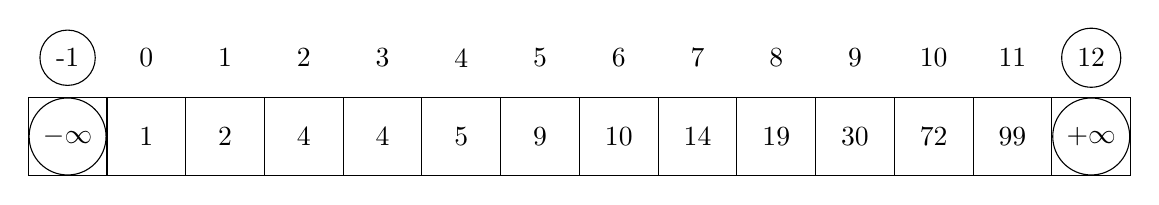
\begin{tikzpicture}
\draw[black] (-1,0) grid (13,1);
\node[circle,draw] at (-0.5,0.5) {$-\infty$};
\node at (0.5,0.5) {1};
\node at (1.5,0.5) {2};
\node at (2.5,0.5) {4};
\node at (3.5,0.5) {4};
\node at (4.5,0.5) {5};
\node at (5.5,0.5) {9};
\node at (6.5,0.5) {10};
\node at (7.5,0.5) {14};
\node at (8.5,0.5) {19};
\node at (9.5,0.5) {30};
\node at (10.5,0.5) {72};
\node at (11.5,0.5) {99};
\node[circle,draw] at (12.5,0.5) {$+\infty$};
\node[circle,draw] at (-0.5,1.5) {-1};
\node at (0.5,1.5) {0};
\node at (1.5,1.5) {1};
\node at (2.5,1.5) {2};
\node at (3.5,1.5) {3};
\node at (4.5,1.5) {4};
\node at (5.5,1.5) {5};
\node at (6.5,1.5) {6};
\node at (7.5,1.5) {7};
\node at (8.5,1.5) {8};
\node at (9.5,1.5) {9};
\node at (10.5,1.5) {10};
\node at (11.5,1.5) {11};
\node[circle,draw] at (12.5,1.5) {12};
\end{tikzpicture}
\end{center}

\begin{center}
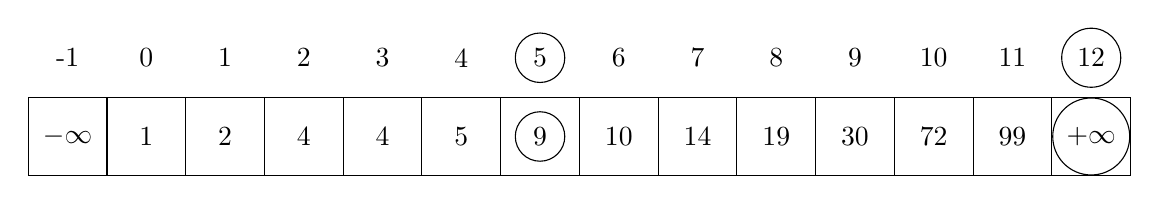
\begin{tikzpicture}
\draw[black] (-1,0) grid (13,1);
\node at (-0.5,0.5) {$-\infty$};
\node at (0.5,0.5) {1};
\node at (1.5,0.5) {2};
\node at (2.5,0.5) {4};
\node at (3.5,0.5) {4};
\node at (4.5,0.5) {5};
\node[circle,draw] at (5.5,0.5) {9};
\node at (6.5,0.5) {10};
\node at (7.5,0.5) {14};
\node at (8.5,0.5) {19};
\node at (9.5,0.5) {30};
\node at (10.5,0.5) {72};
\node at (11.5,0.5) {99};
\node[circle,draw] at (12.5,0.5) {$+\infty$};
\node at (-0.5,1.5) {-1};
\node at (0.5,1.5) {0};
\node at (1.5,1.5) {1};
\node at (2.5,1.5) {2};
\node at (3.5,1.5) {3};
\node at (4.5,1.5) {4};
\node[circle,draw] at (5.5,1.5) {5};
\node at (6.5,1.5) {6};
\node at (7.5,1.5) {7};
\node at (8.5,1.5) {8};
\node at (9.5,1.5) {9};
\node at (10.5,1.5) {10};
\node at (11.5,1.5) {11};
\node[circle,draw] at (12.5,1.5) {12};
\end{tikzpicture}
\end{center}

\begin{center}
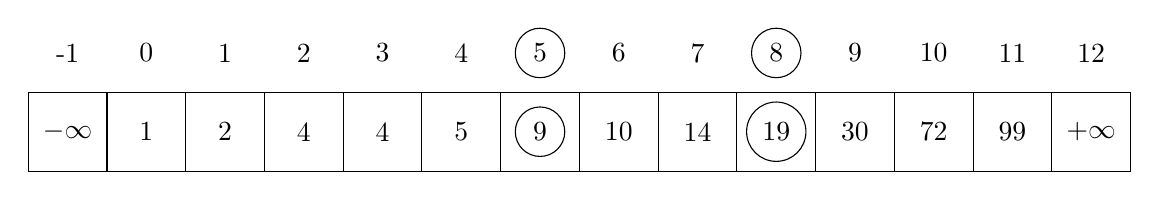
\begin{tikzpicture}
\draw[black] (-1,0) grid (13,1);
\node at (-0.5,0.5) {$-\infty$};
\node at (0.5,0.5) {1};
\node at (1.5,0.5) {2};
\node at (2.5,0.5) {4};
\node at (3.5,0.5) {4};
\node at (4.5,0.5) {5};
\node[circle,draw] at (5.5,0.5) {9};
\node at (6.5,0.5) {10};
\node at (7.5,0.5) {14};
\node[circle,draw] at (8.5,0.5) {19};
\node at (9.5,0.5) {30};
\node at (10.5,0.5) {72};
\node at (11.5,0.5) {99};
\node at (12.5,0.5) {$+\infty$};
\node at (-0.5,1.5) {-1};
\node at (0.5,1.5) {0};
\node at (1.5,1.5) {1};
\node at (2.5,1.5) {2};
\node at (3.5,1.5) {3};
\node at (4.5,1.5) {4};
\node[circle,draw] at (5.5,1.5) {5};
\node at (6.5,1.5) {6};
\node at (7.5,1.5) {7};
\node[circle,draw] at (8.5,1.5) {8};
\node at (9.5,1.5) {9};
\node at (10.5,1.5) {10};
\node at (11.5,1.5) {11};
\node at (12.5,1.5) {12};
\end{tikzpicture}
\end{center}

\begin{center}
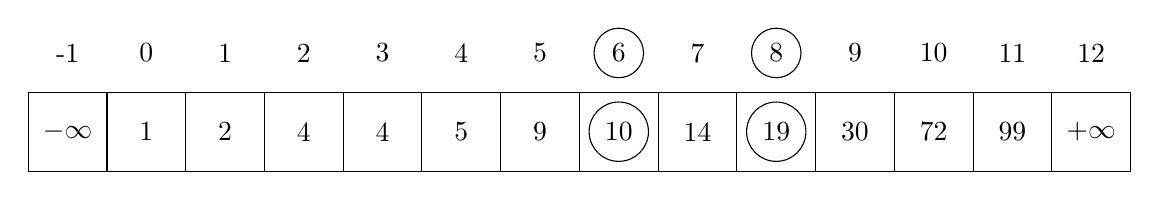
\begin{tikzpicture}
\draw[black] (-1,0) grid (13,1);
\node at (-0.5,0.5) {$-\infty$};
\node at (0.5,0.5) {1};
\node at (1.5,0.5) {2};
\node at (2.5,0.5) {4};
\node at (3.5,0.5) {4};
\node at (4.5,0.5) {5};
\node at (5.5,0.5) {9};
\node[circle,draw] at (6.5,0.5) {10};
\node at (7.5,0.5) {14};
\node[circle,draw] at (8.5,0.5) {19};
\node at (9.5,0.5) {30};
\node at (10.5,0.5) {72};
\node at (11.5,0.5) {99};
\node at (12.5,0.5) {$+\infty$};
\node at (-0.5,1.5) {-1};
\node at (0.5,1.5) {0};
\node at (1.5,1.5) {1};
\node at (2.5,1.5) {2};
\node at (3.5,1.5) {3};
\node at (4.5,1.5) {4};
\node at (5.5,1.5) {5};
\node[circle,draw] at (6.5,1.5) {6};
\node at (7.5,1.5) {7};
\node[circle,draw] at (8.5,1.5) {8};
\node at (9.5,1.5) {9};
\node at (10.5,1.5) {10};
\node at (11.5,1.5) {11};
\node at (12.5,1.5) {12};
\end{tikzpicture}
\end{center}

\begin{center}
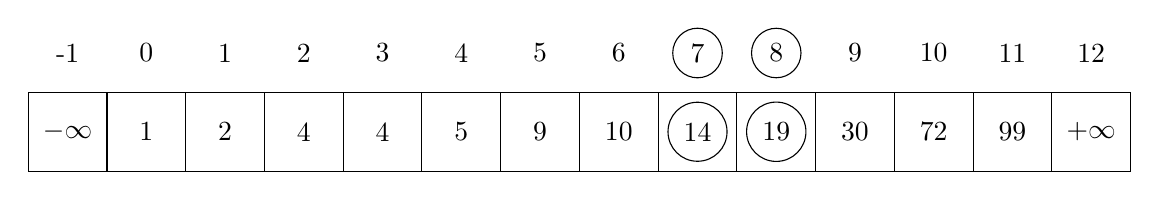
\begin{tikzpicture}
\draw[black] (-1,0) grid (13,1);
\node at (-0.5,0.5) {$-\infty$};
\node at (0.5,0.5) {1};
\node at (1.5,0.5) {2};
\node at (2.5,0.5) {4};
\node at (3.5,0.5) {4};
\node at (4.5,0.5) {5};
\node at (5.5,0.5) {9};
\node at (6.5,0.5) {10};
\node[circle,draw] at (7.5,0.5) {14};
\node[circle,draw] at (8.5,0.5) {19};
\node at (9.5,0.5) {30};
\node at (10.5,0.5) {72};
\node at (11.5,0.5) {99};
\node at (12.5,0.5) {$+\infty$};
\node at (-0.5,1.5) {-1};
\node at (0.5,1.5) {0};
\node at (1.5,1.5) {1};
\node at (2.5,1.5) {2};
\node at (3.5,1.5) {3};
\node at (4.5,1.5) {4};
\node at (5.5,1.5) {5};
\node at (6.5,1.5) {6};
\node[circle,draw] at (7.5,1.5) {7};
\node[circle,draw] at (8.5,1.5) {8};
\node at (9.5,1.5) {9};
\node at (10.5,1.5) {10};
\node at (11.5,1.5) {11};
\node at (12.5,1.5) {12};
\end{tikzpicture}
\end{center}

最終的に\texttt{ub == 8}となる。
\texttt{A[lb] < x} と \texttt{A[ub] >= x}が常に満たされていることに注意しよう。
\textbf{このように覚えておけば二分探索のプログラムを忘れることはない}。
二分探索はとても応用が広く、様々な問題を解くのに使うことができる。
その場合に特にこの覚えやすい二分探索の書き方が役に立つ。


\section{二分探索の応用}
二分探索はソートされた配列から値を探すという目的以外にも使用することができる。
ソートされた配列の代わりに単調な二値関数$p\colon \{0,1,2,\dotsc,n-1\}\to\{0,1\}$について考えよう。
ここで$p$が単調というのは$p(x)\ge p(x-1)$が$x=1,2,\dotsc,n-1$について満たされるという意味である。
このような$p$について
\begin{center}
$p(x) = 1$を満たす最小の$x\in\{0,1,2,\dotsc,n-1\}$をもとめよ
\end{center}
という問題を二分探索で解くことができる。
具体的には次のようなプログラムになる。

\begin{minipage}{\linewidth}
\begin{lstlisting}[basicstyle=\ttfamily\normalsize,showstringspaces=false,language=C,frame=single]
int lb, ub;
lb = 「絶対にp(lb) == 0となる値」;
ub = 「絶対にp(ub) == 1となる値」;
while(ub - lb > 1) {
  int mid = (lb + ub) / 2;
  if(p(mid)){
    ub = mid;
  }
  else {
    lb = mid;
  }
}
/* ここで ub が p(ub) == 1 となる最小の値
          lb が p(lb) == 0 となる最大の値となっている */
\end{lstlisting}
\end{minipage}
この考え方を用いると、上記の問題について非常に大きな$n$に対しても現実的な時間で解くことができる。

例えば簡単な例として整数$n$の平方根の切り上げ$\lceil \sqrt{n}\rceil$を求める問題を考えよう。
この場合、
\begin{equation*}
p(x) :=
\begin{cases}
1,& \text{if } x \ge \sqrt{n}\\
0,& \text{otherwise}
\end{cases}
\end{equation*}
とすると、$p(x)=1$となる最小の整数$x$が$\lceil\sqrt{n}\rceil$である。これを次のように書き換えることができる。
\begin{equation*}
p(x) =
\begin{cases}
1,& \text{if } x^2 \ge n\\
0,& \text{otherwise}
\end{cases}
\end{equation*}
よって、
\begin{lstlisting}[basicstyle=\ttfamily\normalsize,showstringspaces=false,language=C,frame=single]
int p(unsigned int x){
  return x * x >= n;
}
\end{lstlisting}
と定義してあげれば、二分探索で$\lceil \sqrt{n}\rceil$が計算できる。
変数\texttt{lb}と\texttt{ub}の初期値は\texttt{lb = 0}, \texttt{ub = n}とすればよい(もちろん、もっと良い$\lceil\sqrt{n}\rceil$の上下界を使ってもよい)。
そうすると反復回数は$\lceil\log n\rceil$である。
このように、\textbf{簡単に計算ができる単調な関数の逆関数は二分探索を用いて計算ができる}。
今回は整数だけを考えているが、実数にも簡単に一般化できる。
その場合\texttt{lb, ub, mid}は \texttt{unsigned int} ではなく \texttt{double} という型にする必要がある。

\begin{minipage}{\linewidth}
\begin{lstlisting}[basicstyle=\ttfamily\normalsize,showstringspaces=false,language=C,frame=single]
unsigned int p(double a, double x){
  return a * a >= x;
}

/* x は非負 */
double sqrt(double x){
  double lb, ub;
  if(x <= 1){
    lb = 0;
    ub = 1;
  }
  else {
    lb = 1;
    ub = x; /* もっといい上界を使ってもいい */
  }
  while(ub - lb > 0.000001){
    double mid = (lb + ub) / 2;
    if(p(mid, x)) ub = mid;
    else lb = mid;
  }
  return (lb + ub) / 2;
}
\end{lstlisting}
\end{minipage}
この関数\texttt{sqrt}は引数の平方根を\texttt{0.000001}の半分以下の誤差で返す。
ここで、\texttt{ub - lb > 0.000001} をループの条件としているが、
浮動小数演算の桁落ちのせいで、\texttt{ub}や\texttt{lb}がとても大きいときに、数値誤差の影響でループが停止しないことがあるため危険である。
そこで、決まった回数だけループするという方法も一般的である。
例えば20回反復すれば、最初の誤差(\texttt{x <= 1}なら\texttt{1}、そうでなければ\texttt{x-1})の$2^{21}$分の一の誤差になる。
一方で平方根の計算にはニュートン法というもっと効率的な方法が存在する。
しかしニュートン法は関数(この場合$x^2$にあたるもの)の凸性も用いるので、単調性しか必要としない二分探索の方が適用範囲が広い。

\section{二分法}
二分探索と非常に良く似たアルゴリズムに「二分法」がある。
これは\textbf{連続関数}の零点の一つを計算するためのアルゴリズムである。
連続関数$f\colon\mathbb{R}\to\mathbb{R}$の零点の一つを計算することを考える。
ある$y>x$について、$f(x)$と$f(y)$の符号が違うとき、ある$z\in(x,y)$が存在して$f(z)=0$となる(中間値の定理)。
よって、まず最初に$f(x)$と$f(y)$の符号が異なるような$x$と$y$を知っていれば、$m=(x+y)/2$について$f(m)$を評価し、
その符号によって$(x, m)$もしくは$(m, y)$のどちらかについて零点が必ず存在することが分かる。
二分探索と同様に1ステップで区間が半分になるので$n$ステップ実行すれば、$(y-x)/2^{n+1}$の誤差で零点が計算できる。

二分法を適用するために必要な$f$の性質は「連続性」である。一方、二分探索に必要な$p$の性質は「単調性」である。
そのため、二分探索と区別して上記のアルゴリズムを二分法と呼ぶことにする。
あまり区別しないで両方二分探索と呼んでいる人も少なくない。


\section{全体のC言語プログラム}
%前回説明したように単調な関数$p\colon \mathbb{Z}\to\{0,1\}$について、$p(z)=1$となる最小の$z\in\mathbb{Z}$を見つける二分探索のプログラムは次のようになる。

例えば入力として整数$n\ge 1$をとり、$\lceil\sqrt{n}\rceil$を出力するプログラムは次のようになる。

\begin{minipage}{\linewidth}
\begin{lstlisting}[basicstyle=\ttfamily\normalsize,showstringspaces=false,language=C,frame=single]
#include <stdio.h>

int n;

int p(int m){
  return (long long int) m * m >= n;
}

int main(){
  int lb, ub;
  scanf("%d", &n);
  lb = 0;
  ub = n;
  while(ub - lb > 1) {
    int mid = (lb + ub) / 2;
    if(p(mid)){
      ub = mid;
    }
    else {
      lb = mid;
    }
  }
  printf("%d\n", ub);
  return 0;
}
\end{lstlisting}
\end{minipage}

\begin{itemize}
\item \texttt{\#include <stdio.h>} は毎回書くおまじない。入出力関係のライブラリを使うためのヘッダファイルの取り込み。これが無いと\texttt{scanf}や\texttt{printf}が使えない。
\item \texttt{int n;} のような関数の外側にある変数は\textbf{グローバル変数}と呼ばれ、プログラムのどこからでもアクセスできる。明示的に初期化しない場合は\textbf{0で初期化}されている。
\item \texttt{int main()} は\textbf{main関数}という特別な関数で、プログラムを実行するとこのmain関数が実行される。
\item \texttt{int lb, ub;} のような関数の内側にある変数は\textbf{ローカル変数}と呼ばれ、その関数の内側からだけアクセスできる。明示的に初期化しない場合は\textbf{どのような値になっているか保証はない}。必ず初期化をすること。
\item \texttt{scanf("\%d", \&n);} は\textbf{標準入力から整数を読み込み}\texttt{n}に代入する命令文である。
標準入力から整数を2つ読み込んで\texttt{int}型の変数\texttt{a}と\texttt{b}に代入したい場合は\texttt{scanf("\%d\%d", \&a, \&b);} とする。
\item \texttt{printf("\%d\textbackslash n", \&n);} は標準出力へ整数\texttt{n}と改行コード \texttt{\textbackslash n}を出力する。
\item \texttt{return 0;} はmain関数の最後に書いておこう(書かなくてもエラーが起きる訳ではないが)。これは「プログラムが正常に終了した」ということを表わしている。
エラーで終了するときは\texttt{return 1;}など0以外の値を返すようにする。この授業ではエラーによる終了は扱わないので、main関数の最後に\texttt{return 0;}を書くことを覚えておけばよい。
\end{itemize}
他によくある処理として、最初に数列の長さ$n$を、その後に数列$A_0,\dotsc,A_{n-1}$を読み込みたい場合は
\begin{lstlisting}[basicstyle=\ttfamily\normalsize,showstringspaces=false,language=C,frame=single]
int i, n;
scanf("%d", &n);
for(i = 0; i < n; i++){
  scanf("%d", &A[i]);
}
\end{lstlisting}
とする。
ここで
\begin{lstlisting}[basicstyle=\ttfamily\normalsize,showstringspaces=false,language=C,frame=single]
for(AAA; BBB; CCC){
  DDD
}
\end{lstlisting}
は
\begin{lstlisting}[basicstyle=\ttfamily\normalsize,showstringspaces=false,language=C,frame=single]
AAA;
while(BBB){
  DDD
  CCC;
}
\end{lstlisting}
と等価である。
ここで、\texttt{AAA, BBB, CCC} はそれぞれ一つの文であり、\texttt{DDD}は文の列であるとする。

標準入力とは特定のファイルなどではなくプログラムが受け付ける入力であり、\texttt{scanf}を用いたプログラムを
実行すると入力受け付け状態になる。入力と改行(Enterキー)を入力すると、\texttt{scanf}により読み取られて残りの処理が実行される。
毎回入力するのが面倒くさい場合はターミナルで \texttt{echo 100 | ./a.out} とすれば \texttt{./a.out} としてから 100 を入力してEnterを押すのと同じことになる。
また、ファイル\texttt{file.txt}に入力を記入しておいてから、\texttt{./a.out < file.txt} としてもよい。

\section{より高度な二分探索}
二分探索とは、単調な関数$p\colon \mathbb{Z}\to\{0,1\}$について、$p(x)=1$となる最小の$x\in\mathbb{Z}$を見つけるアルゴリズムであった。
この二分探索は適用範囲が広く、様々な応用がある。
例えば、今回の課題(後述)の「りんご狩り」では
\begin{equation*}
p(x) := \begin{cases}
1,& \text{if $x$個のりんごが入るりんごバッグを合計$k$個配ると全員がりんごを持って帰れる}\\
0,& \text{otherwise.}
\end{cases}
\end{equation*}
と定義すれば$p$は単調性を満たし、$p(x)=1$となる最小の$x$が求める解となる。
この$p(x)$は効率的に計算することができるので、この問題を十分効率的に解くことができる。



\section{課題}\label{sec:assign}
以下のすべての課題について、二分探索で用いる\texttt{lb} と\texttt{ub} の初期値はできるだけ良いものを選ぶこと。
\texttt{lb+1}や\texttt{ub-1}が初期値として使用できないようなものを選ぶこと。
最初の配列の問題以外は入力に依存しない初期値を考えればよい。入力制約に注意すること。
また、二分探索における$p$の評価は$O(n)$回の演算(整数の四則演算、比較)でおこなうこと。ここでいう$n$は各問題の入力に現れる$n$である。

\clearpage
\subsection{配列の二分探索 $\bigstar$}
\begin{itembox}[l]{問題文}
単調非減少整数列$a_0, a_1,\dotsc, a_{n-1}$と整数$k$について、$a_x\ge k$となる最小の整数$x$を求めよ。
ただし、そのような$x$が存在しないときは$x=n$とする。
\end{itembox}

\begin{itembox}[l]{入力制約}
$1\le n\le 10^5$\\
$1\le k\le 10^9$\\
$1\le a_i\le 10^9$,\hspace{2em} $i\in\{0,1,\dotsc,n-1\}$\\
$a_i\le a_{i+1}$,\hspace{2em} $i\in\{0,1,\dotsc,n-2\}$
\end{itembox}

\begin{itembox}[l]{入力}
$n~k$\\
$a_0~a_1~\dotsb~a_{n-1}$
\end{itembox}

\begin{itembox}[l]{出力}
$x$
\end{itembox}

\begin{itembox}[l]{サンプル1}
入力:
\begin{verbatim}
12 17
1 2 4 4 5 9 10 14 19 30 72 99
\end{verbatim}
出力:
\begin{verbatim}
8
\end{verbatim}
\end{itembox}

\begin{itembox}[l]{サンプル2}
入力:
\begin{verbatim}
12 3
1 2 4 4 5 9 10 14 19 30 72 99
\end{verbatim}
出力:
\begin{verbatim}
2
\end{verbatim}
\end{itembox}

\begin{itembox}[l]{サンプル3}
入力:
\begin{verbatim}
1 10
9
\end{verbatim}
出力:
\begin{verbatim}
1
\end{verbatim}
\end{itembox}

\clearpage
\subsection{りんご狩り $\bigstar\bigstar$}
\begin{itembox}[l]{問題文}
りんご狩りに$n$人集まった。
各$i=1,2,\dotsc,n$について$i$番目の人は$a_i$個のりんごを収穫した。
合計$k$個のりんごバッグ(サイズは全て同じ)を配ると、全ての人はりんごを持ち帰ることができた。
りんごバッグに入れることができるりんごの個数としてあり得るもののうち最小値$x$をもとめよ。
\end{itembox}

\begin{itembox}[l]{入力制約}
$1\le n\le 10^5$\\
$1\le a_i\le 10^9$,\hspace{2em}$i\in\{1,2,\dotsc,n\}$\\
$n\le k\le 10^5$
\end{itembox}

\begin{itembox}[l]{入力}
$n~k$\\
$a_1~a_2~\dotsb~a_n$
\end{itembox}

\begin{itembox}[l]{出力}
$x$
\end{itembox}

\begin{itembox}[l]{サンプル1}
入力:
\begin{verbatim}
5 7
1 2 3 4 5
\end{verbatim}
出力:
\begin{verbatim}
3
\end{verbatim}
\end{itembox}

\begin{itembox}[l]{サンプル2}
入力:
\begin{verbatim}
5 5
10 20 30 40 1000
\end{verbatim}
出力:
\begin{verbatim}
1000
\end{verbatim}
\end{itembox}

\begin{itembox}[l]{サンプル3}
入力:
\begin{verbatim}
7 1000
1 2 3 4 5 6 7
\end{verbatim}
出力:
\begin{verbatim}
1
\end{verbatim}
\end{itembox}


\clearpage
\subsection{槍作り $\bigstar\bigstar$}
\begin{itembox}[l]{問題文}
長さ$m$の木から長さ$x$の木製の槍が$\lfloor m/x\rfloor$本作れる。
今$n$本の木があり、各木の長さは$a_1,a_2,\dotsc,a_n$である。
これらの木から同じ長さの木製の槍を$k$本作りたい。
作ることができる槍の長さの最大値$x$をもとめよ。
\end{itembox}

\begin{itembox}[l]{入力制約}
$1\le n\le 10^5$\\
$1\le a_i\le 10^9$,\hspace{2em}$i\in\{1,2,\dotsc,n\}$\\
$1\le k\le 10^5$
\end{itembox}

\begin{itembox}[l]{入力}
$n~k$\\
$a_1~a_2~\dotsb~a_n$
\end{itembox}

\begin{itembox}[l]{出力}
$x$
\end{itembox}

\begin{itembox}[l]{サンプル1}
入力:
\begin{verbatim}
5 7
1 2 3 4 5
\end{verbatim}
出力:
\begin{verbatim}
1
\end{verbatim}
\end{itembox}

\begin{itembox}[l]{サンプル2}
入力:
\begin{verbatim}
5 5
10 20 30 40 1000
\end{verbatim}
出力:
\begin{verbatim}
200
\end{verbatim}
\end{itembox}

\begin{itembox}[l]{サンプル3}
入力:
\begin{verbatim}
7 1000
1 2 3 4 5 6 7
\end{verbatim}
出力:
\begin{verbatim}
0
\end{verbatim}
\end{itembox}



\clearpage
\subsection{仕事配分 $\bigstar\bigstar$}
\begin{itembox}[l]{問題文}
$n$時間の仕事を$k$人の人に配分したい。
それぞれの人は連続した何時間かを働き、また異なる人が同時に働くことはないものとする。
各時間の仕事量が整数列$a_1,a_2,\dotsc,a_n$で与えられるとき、一番仕事量が多い人の仕事量を最小化するように仕事を配分するとする。
そのような仕事配分をしたとき、一番仕事量が多い人の仕事量$x$をもとめよ。
\end{itembox}

\begin{itembox}[l]{入力制約}
$1\le n\le 10^5$\\
$1\le a_i\le 10^4$,\hspace{2em}$i\in\{1,2,\dotsc,n\}$\\
$1\le k\le n$
\end{itembox}

\begin{itembox}[l]{入力}
$n~k$\\
$a_1~a_2~\dotsb~a_n$
\end{itembox}

\begin{itembox}[l]{出力}
$x$
\end{itembox}

\begin{itembox}[l]{サンプル1}
入力:
\begin{verbatim}
3 2
1 2 4
\end{verbatim}
出力:
\begin{verbatim}
4
\end{verbatim}
\end{itembox}

\begin{itembox}[l]{サンプル2}
入力:
\begin{verbatim}
3 2
1 4 2
\end{verbatim}
出力:
\begin{verbatim}
5
\end{verbatim}
\end{itembox}

\begin{itembox}[l]{サンプル3}
入力:
\begin{verbatim}
5 5
10 20 30 40 1000
\end{verbatim}
出力:
\begin{verbatim}
1000
\end{verbatim}
\end{itembox}



\end{document}
